\documentclass{beamer}
\usepackage[italian]{babel}
\usepackage[utf8]{inputenc}
\usetheme{Berlin}
\usecolortheme{wolverine}
\usepackage{booktabs}
\usepackage{siunitx}
\usepackage{graphicx} 
\usepackage{amsmath}
\usepackage{caption}
\usepackage[italian]{babel}
%\usepackage[utf8]{inputenc
\usepackage[absolute,overlay]{textpos}
\usepackage{multirow}
\usepackage{subfig}

\title{WAVEMETER}
\subtitle{Caratterizzazione di due misuratori di lunghezza d'onda e loro applicazioni}

\author{S.~Bottaro\inst{1} \and L.M.~Perrone\inst{1}}

\institute[Unipi] % (optional, but mostly needed)
{
  \inst{1}%
  Dipartimento di Fisica\\
  Università di Pisa
  }
  
\date{Seminario - 2016}  


\begin{document}

\begin{frame}{ENEL}

\begin{textblock}{12}(-1,3)
\begin{figure}
%\centering\\all'illuminazione \\della stanza. CH2 piccato sul rosso.
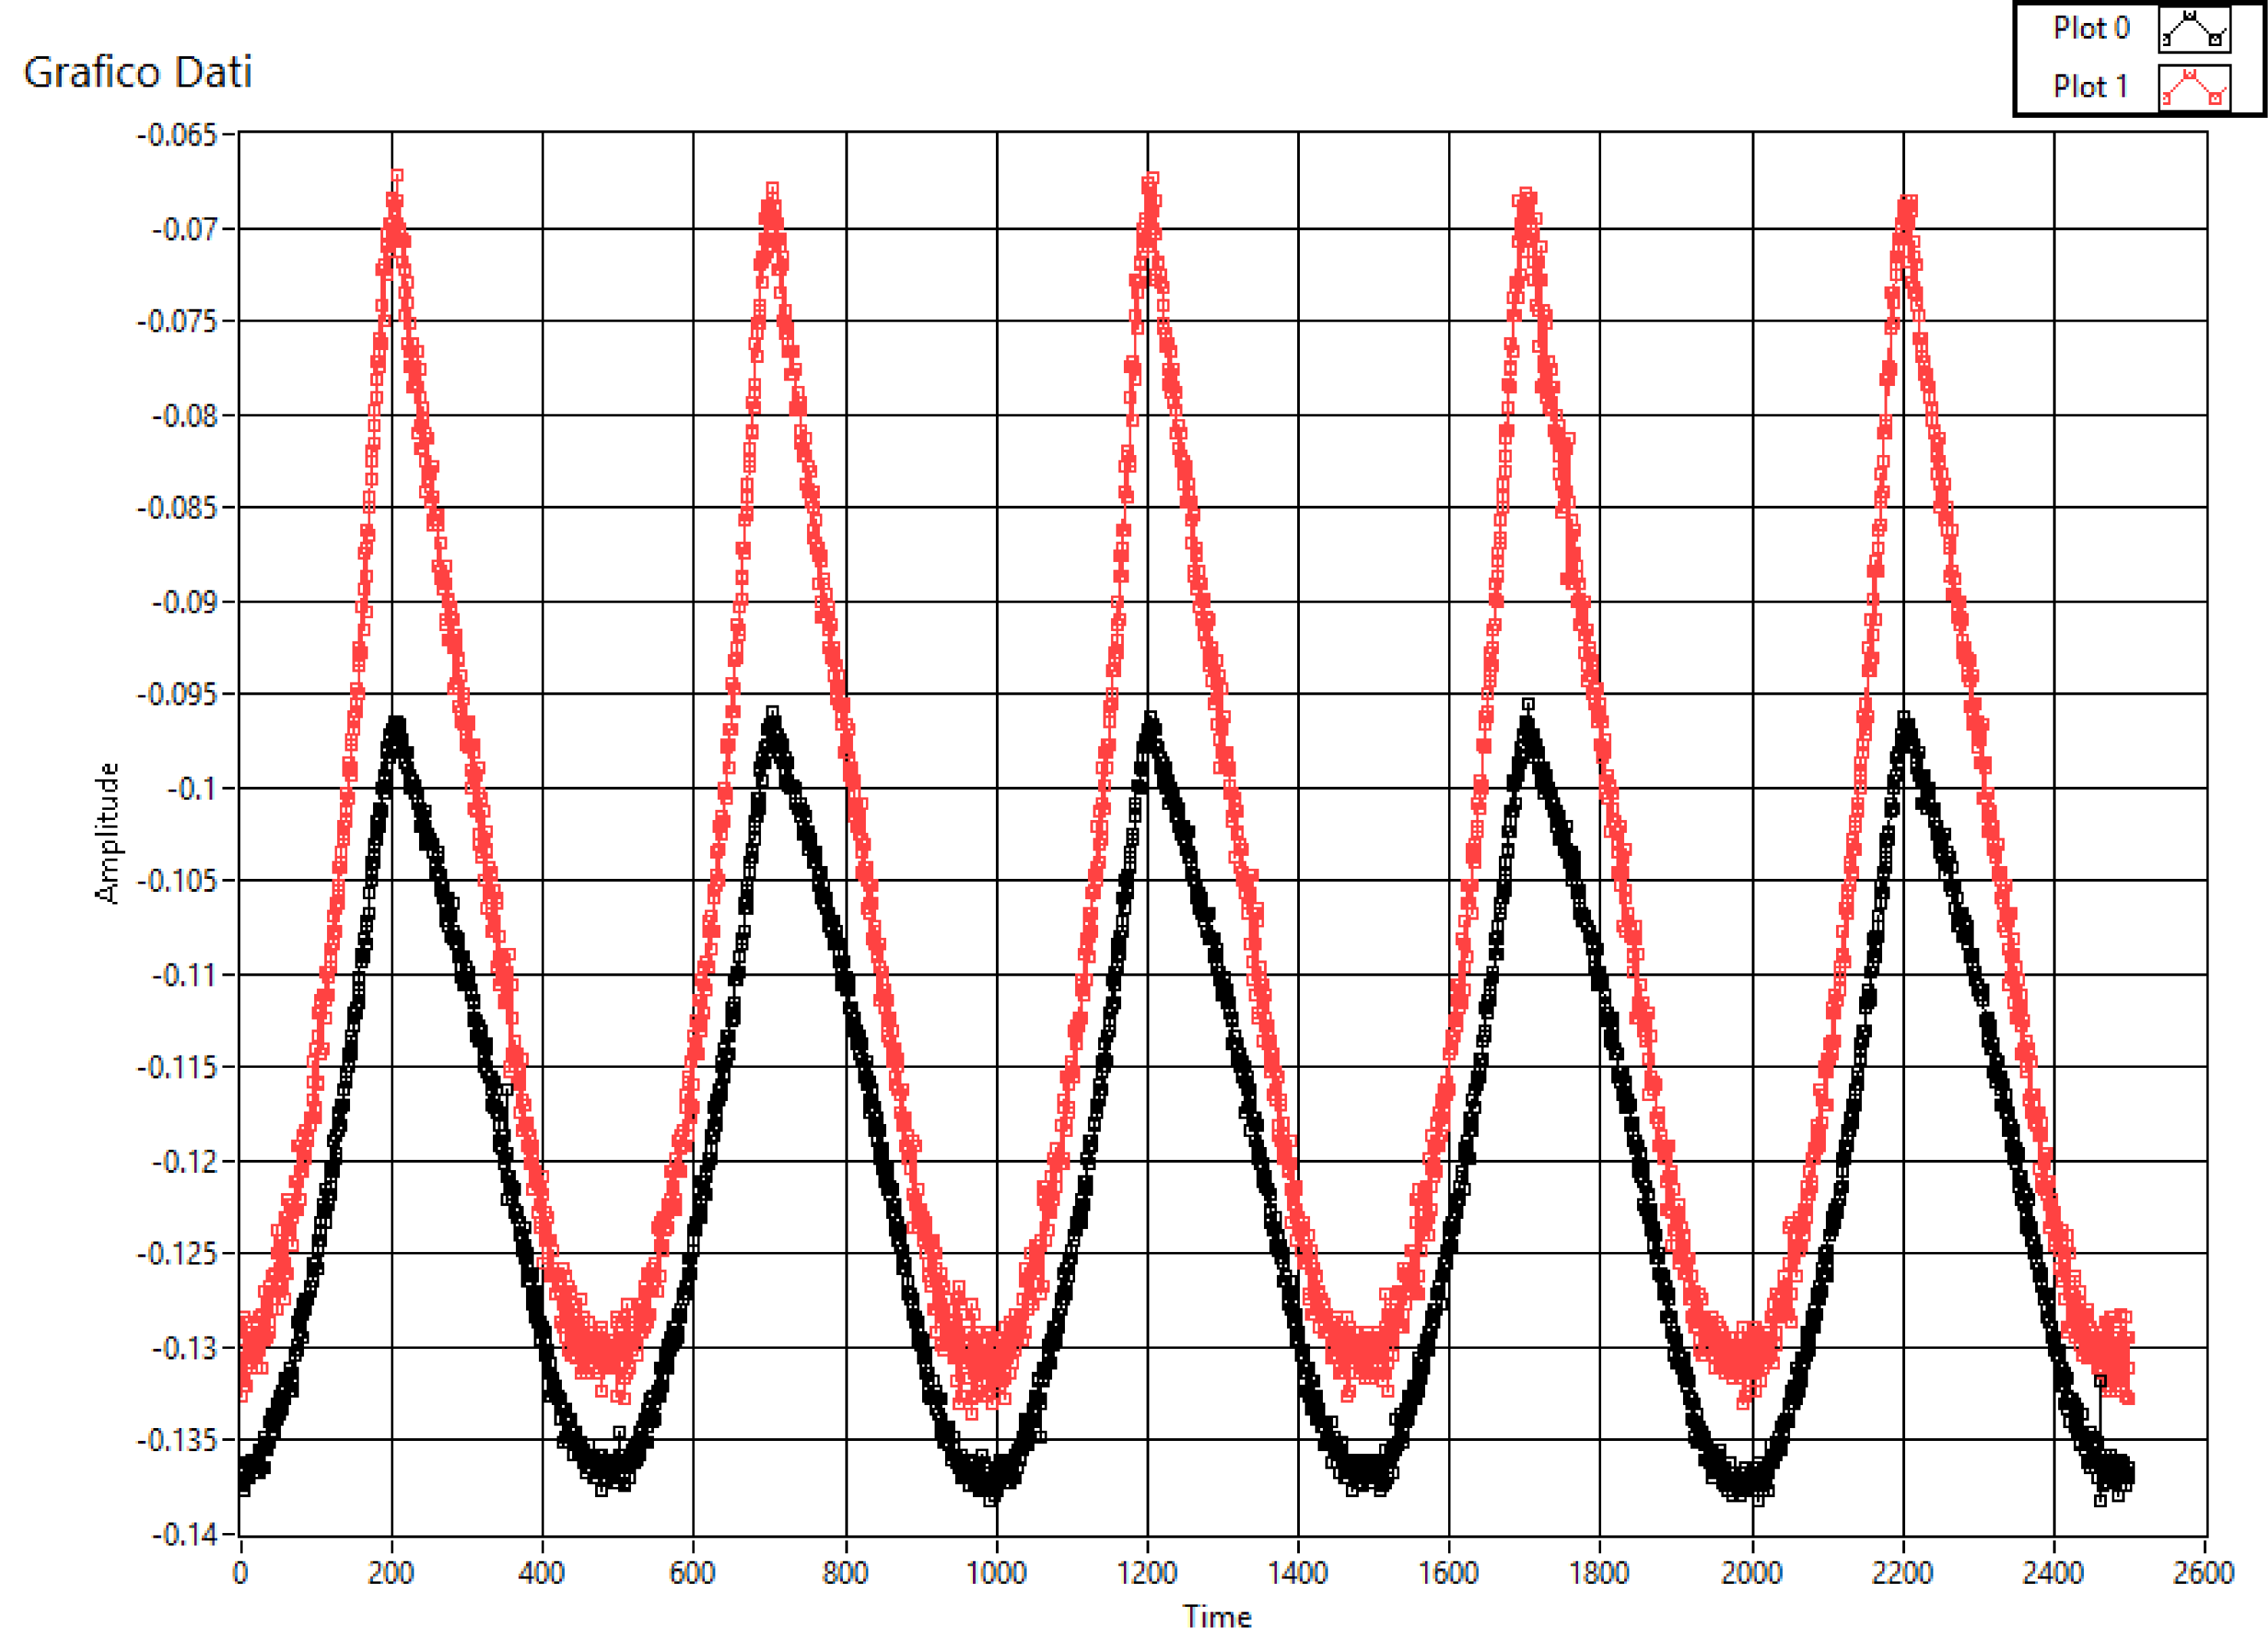
\includegraphics[width=0.5\linewidth]{./luce_stanza_enel}
\caption{Segnale relativo\\
all'illuminazione stanza.}
\label{fig:enel}
\end{figure}
\end{textblock}

\begin{textblock}{12}(6,3)
\begin{figure}
\centering
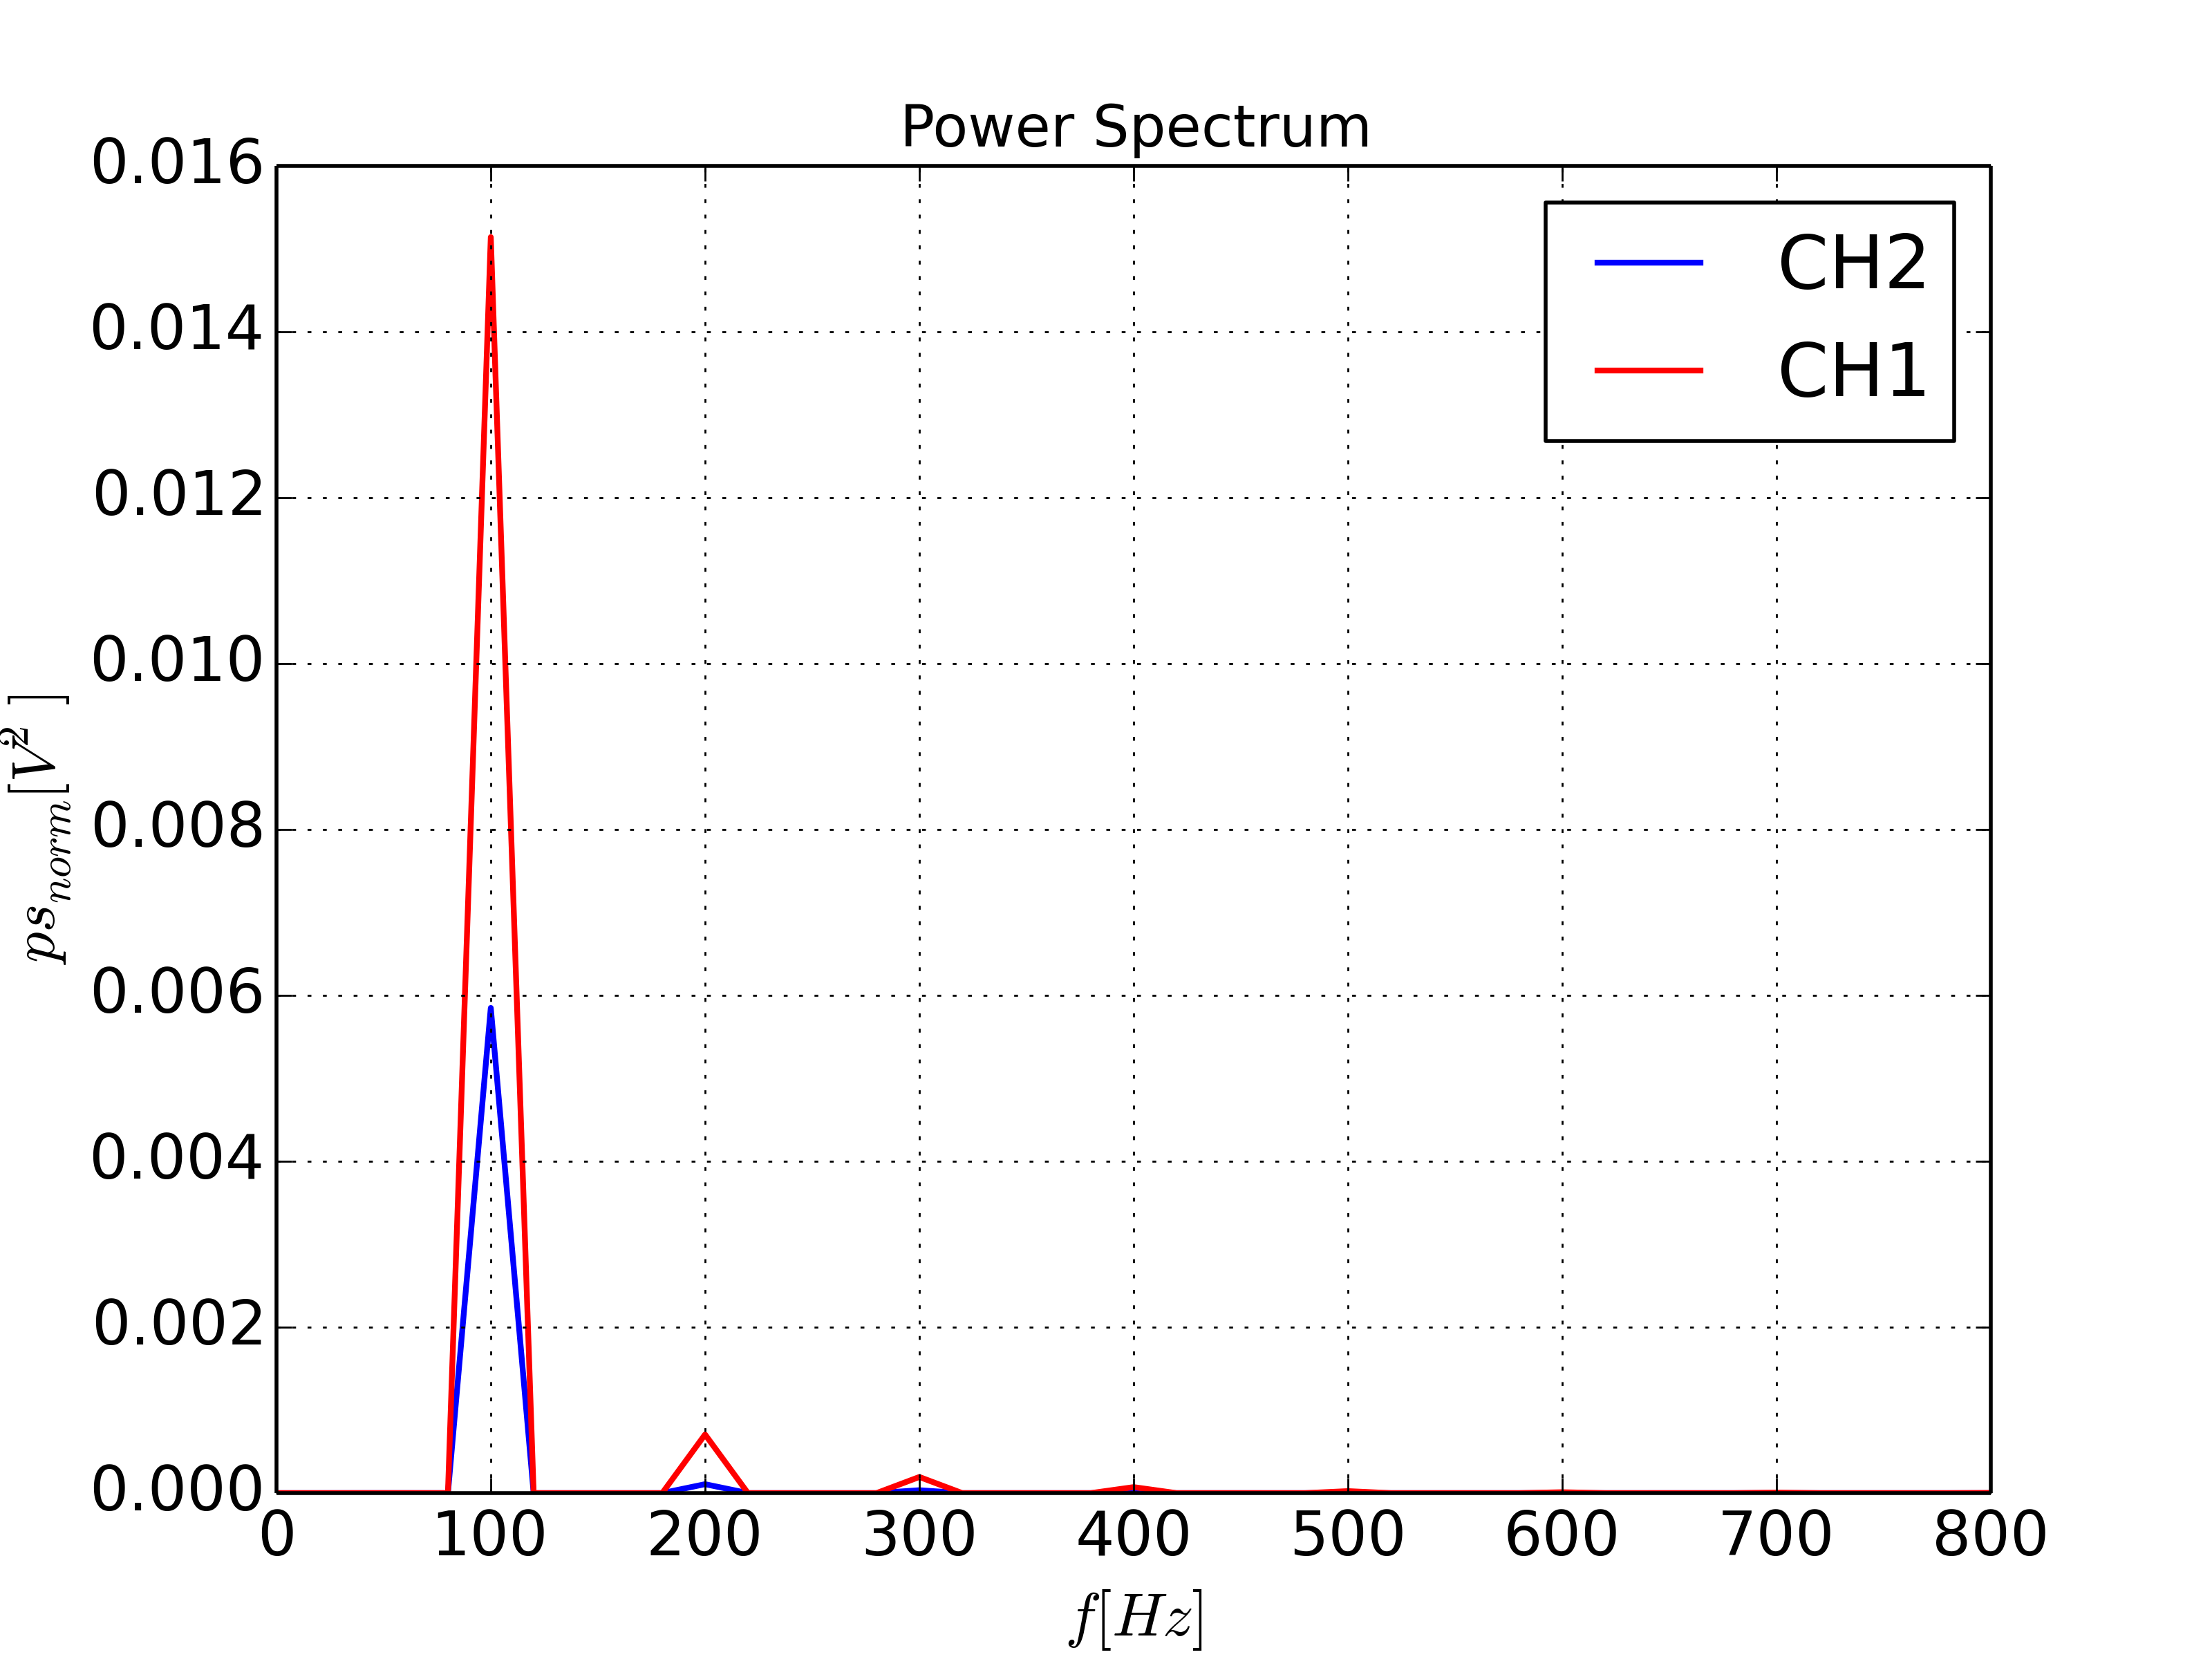
\includegraphics[width=0.5\linewidth]{./fft_lucestanza}
\caption{Fast Fourier transform \\
del segnale di luce ambientale.}
\label{fig:fft_lucestanza}
\end{figure}
\end{textblock}

\begin{textblock}{10}(3,13)
CH2 piccato sul rosso.
\end{textblock}
\end{frame}

\begin{frame}{Montaggio e dimensionamento}
\begin{figure}
\centering
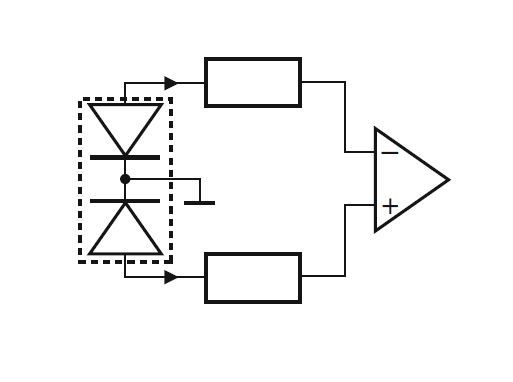
\includegraphics[width=0.35\linewidth]{./circuito_analog}
\caption{Schema di montaggio della coppia di fotodiodi del WS-756-TO5}
\label{fig:schema_montaggio}
\end{figure}

\fontsize{10}{12}
\begin{itemize}
\item Circuito con due op-amp in modalità invertente
\item Due transimpedenze uguali nei limiti dell'errore 
\item Per dimensionare le trans-impedenze si considera la curva di responsività: l'ordine di grandezza della corrente è 10-100 $\mu$A, resistenze a trans-impedenza dell'ordine del centinaio di k$\Omega$
\item $R_1 = 82.3 k\Omega$ e $R_2 = 82.2 k\Omega$ (prima) e $R_1 = 219 k\Omega$ e $R_2 = 220 k\Omega$ (poi).
\end{itemize}
\end{frame}
\begin{frame}{LED impiegati}
\begin{table}[h]
\centering
\fontsize{10}{12}
% This LaTeX table template is generated by emacs 24.3.1
\begin{tabular}{l|c|c|c}
\hline
\textbf{LED} & \textbf{Wavelength} datasheet (nm) & $log(CH1/CH2)$ & $\delta log$ \\
\hline
\textsc{hlmpd101-645} & 645 & -0.539 & 0.006 \\
\textsc{hlmpc115-red} & 637 & -0.522 & 0.003 \\
\textsc{hlmpc315-Y} & 585 & 0.172 & 0.006 \\
\textsc{la3366} & 615 & -0.101 & 0.003 \\
\textsc{lb3333} & 470 & 2.26 & 0.02 \\
\textsc{led450} & 450 & 2.87 & 0.02 \\
\textsc{lo3336} & 606 & -0.101 & 0.002 \\
\textsc{lpk376} & 560 & 0.65 & 0.04 \\
\textsc{ls3336} & 633 & -0.332 & 0.001 \\
\textsc{lt3333} & 528 & 0.908 & 0.01 \\
\textsc{ly3336} & 587 & 0.209 & 0.001 \\
\textsc{sfh4873-880} & 880 & -2.439 & 0.004 \\
\textsc{ssl-lxa} & 660 & -0.58 & 0.02 \\
\textsc{tshg8400-830} & 830 & -1.964 & 0.007 \\
\hline
\end{tabular}
\caption{title}
\label{tabella_LED}
\end{table}

\end{frame}

\begin{frame}{Lunghezze d'onda (datasheet) e curva di calibrazione}
\begin{figure}
\centering
\subfloat[LED ($\lambda$ datasheet) sulla curva di calibrazione del sensore analogico.]{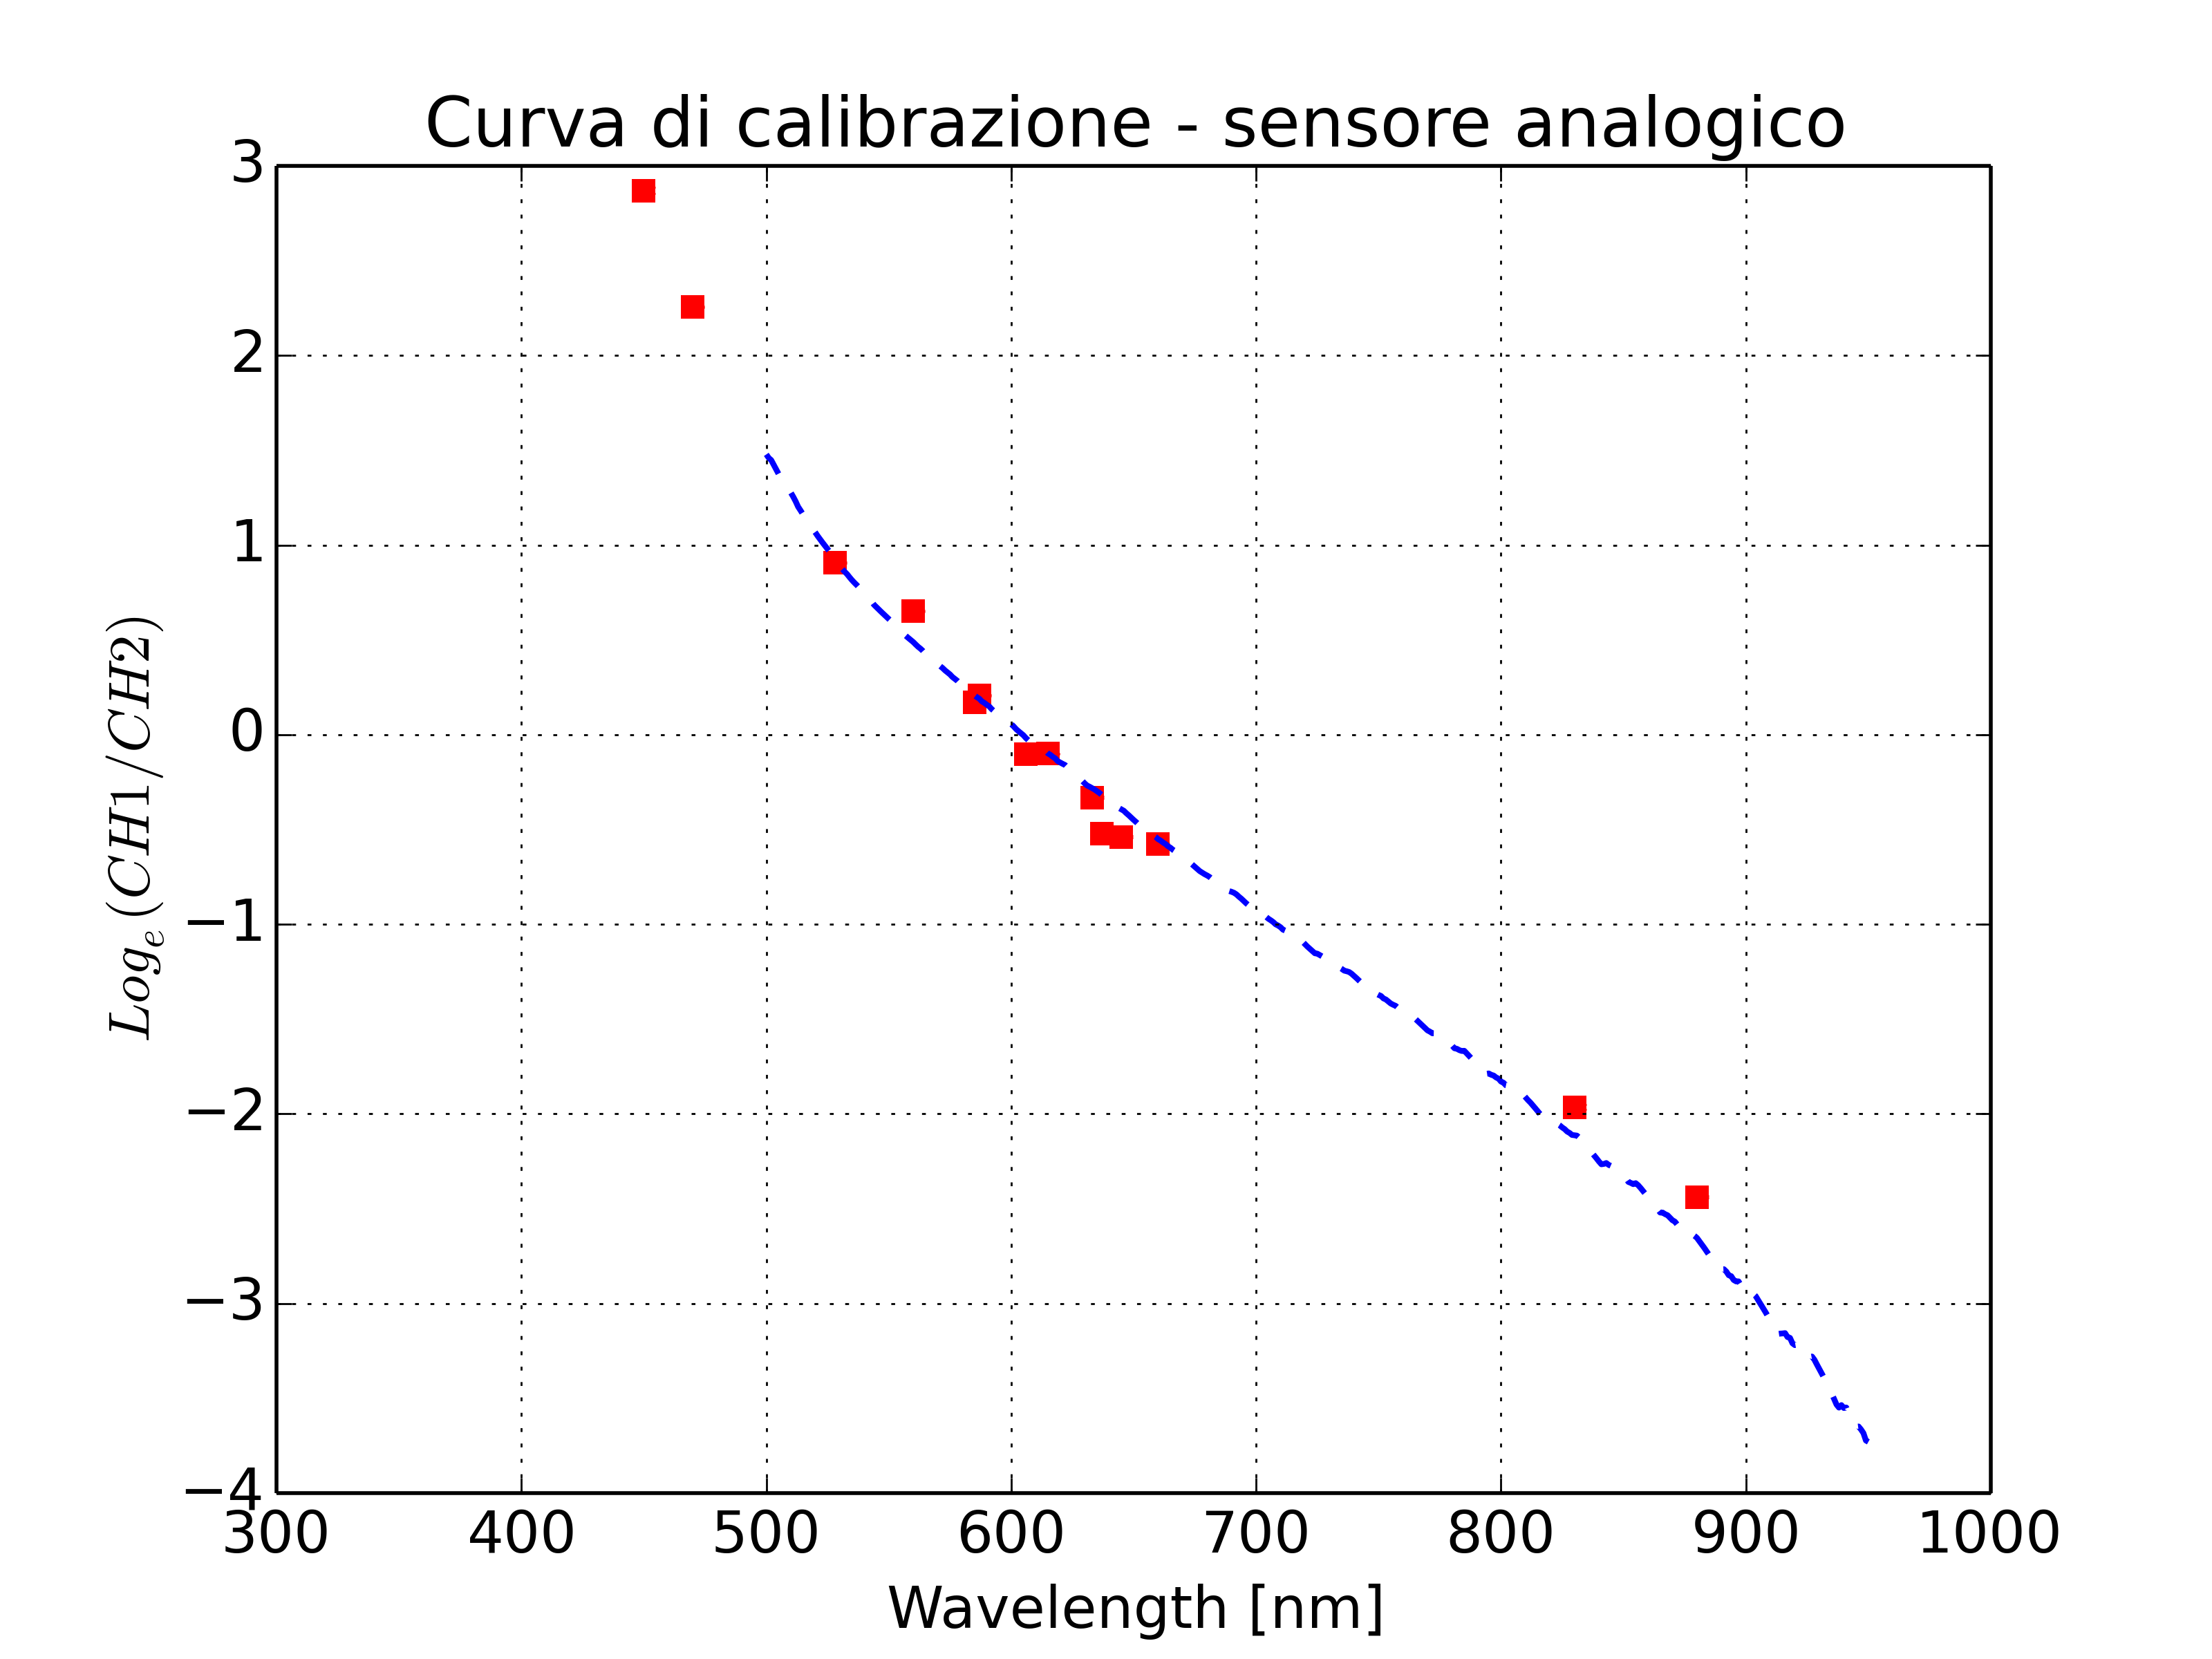
\includegraphics[width=0.4\linewidth]{./calibrazione_led}

\label{fig:calibrazione_led}}
\subfloat[Scarto fra $\lambda$ datasheet e "calibrazione" (interpolate) per ciascun LED.]{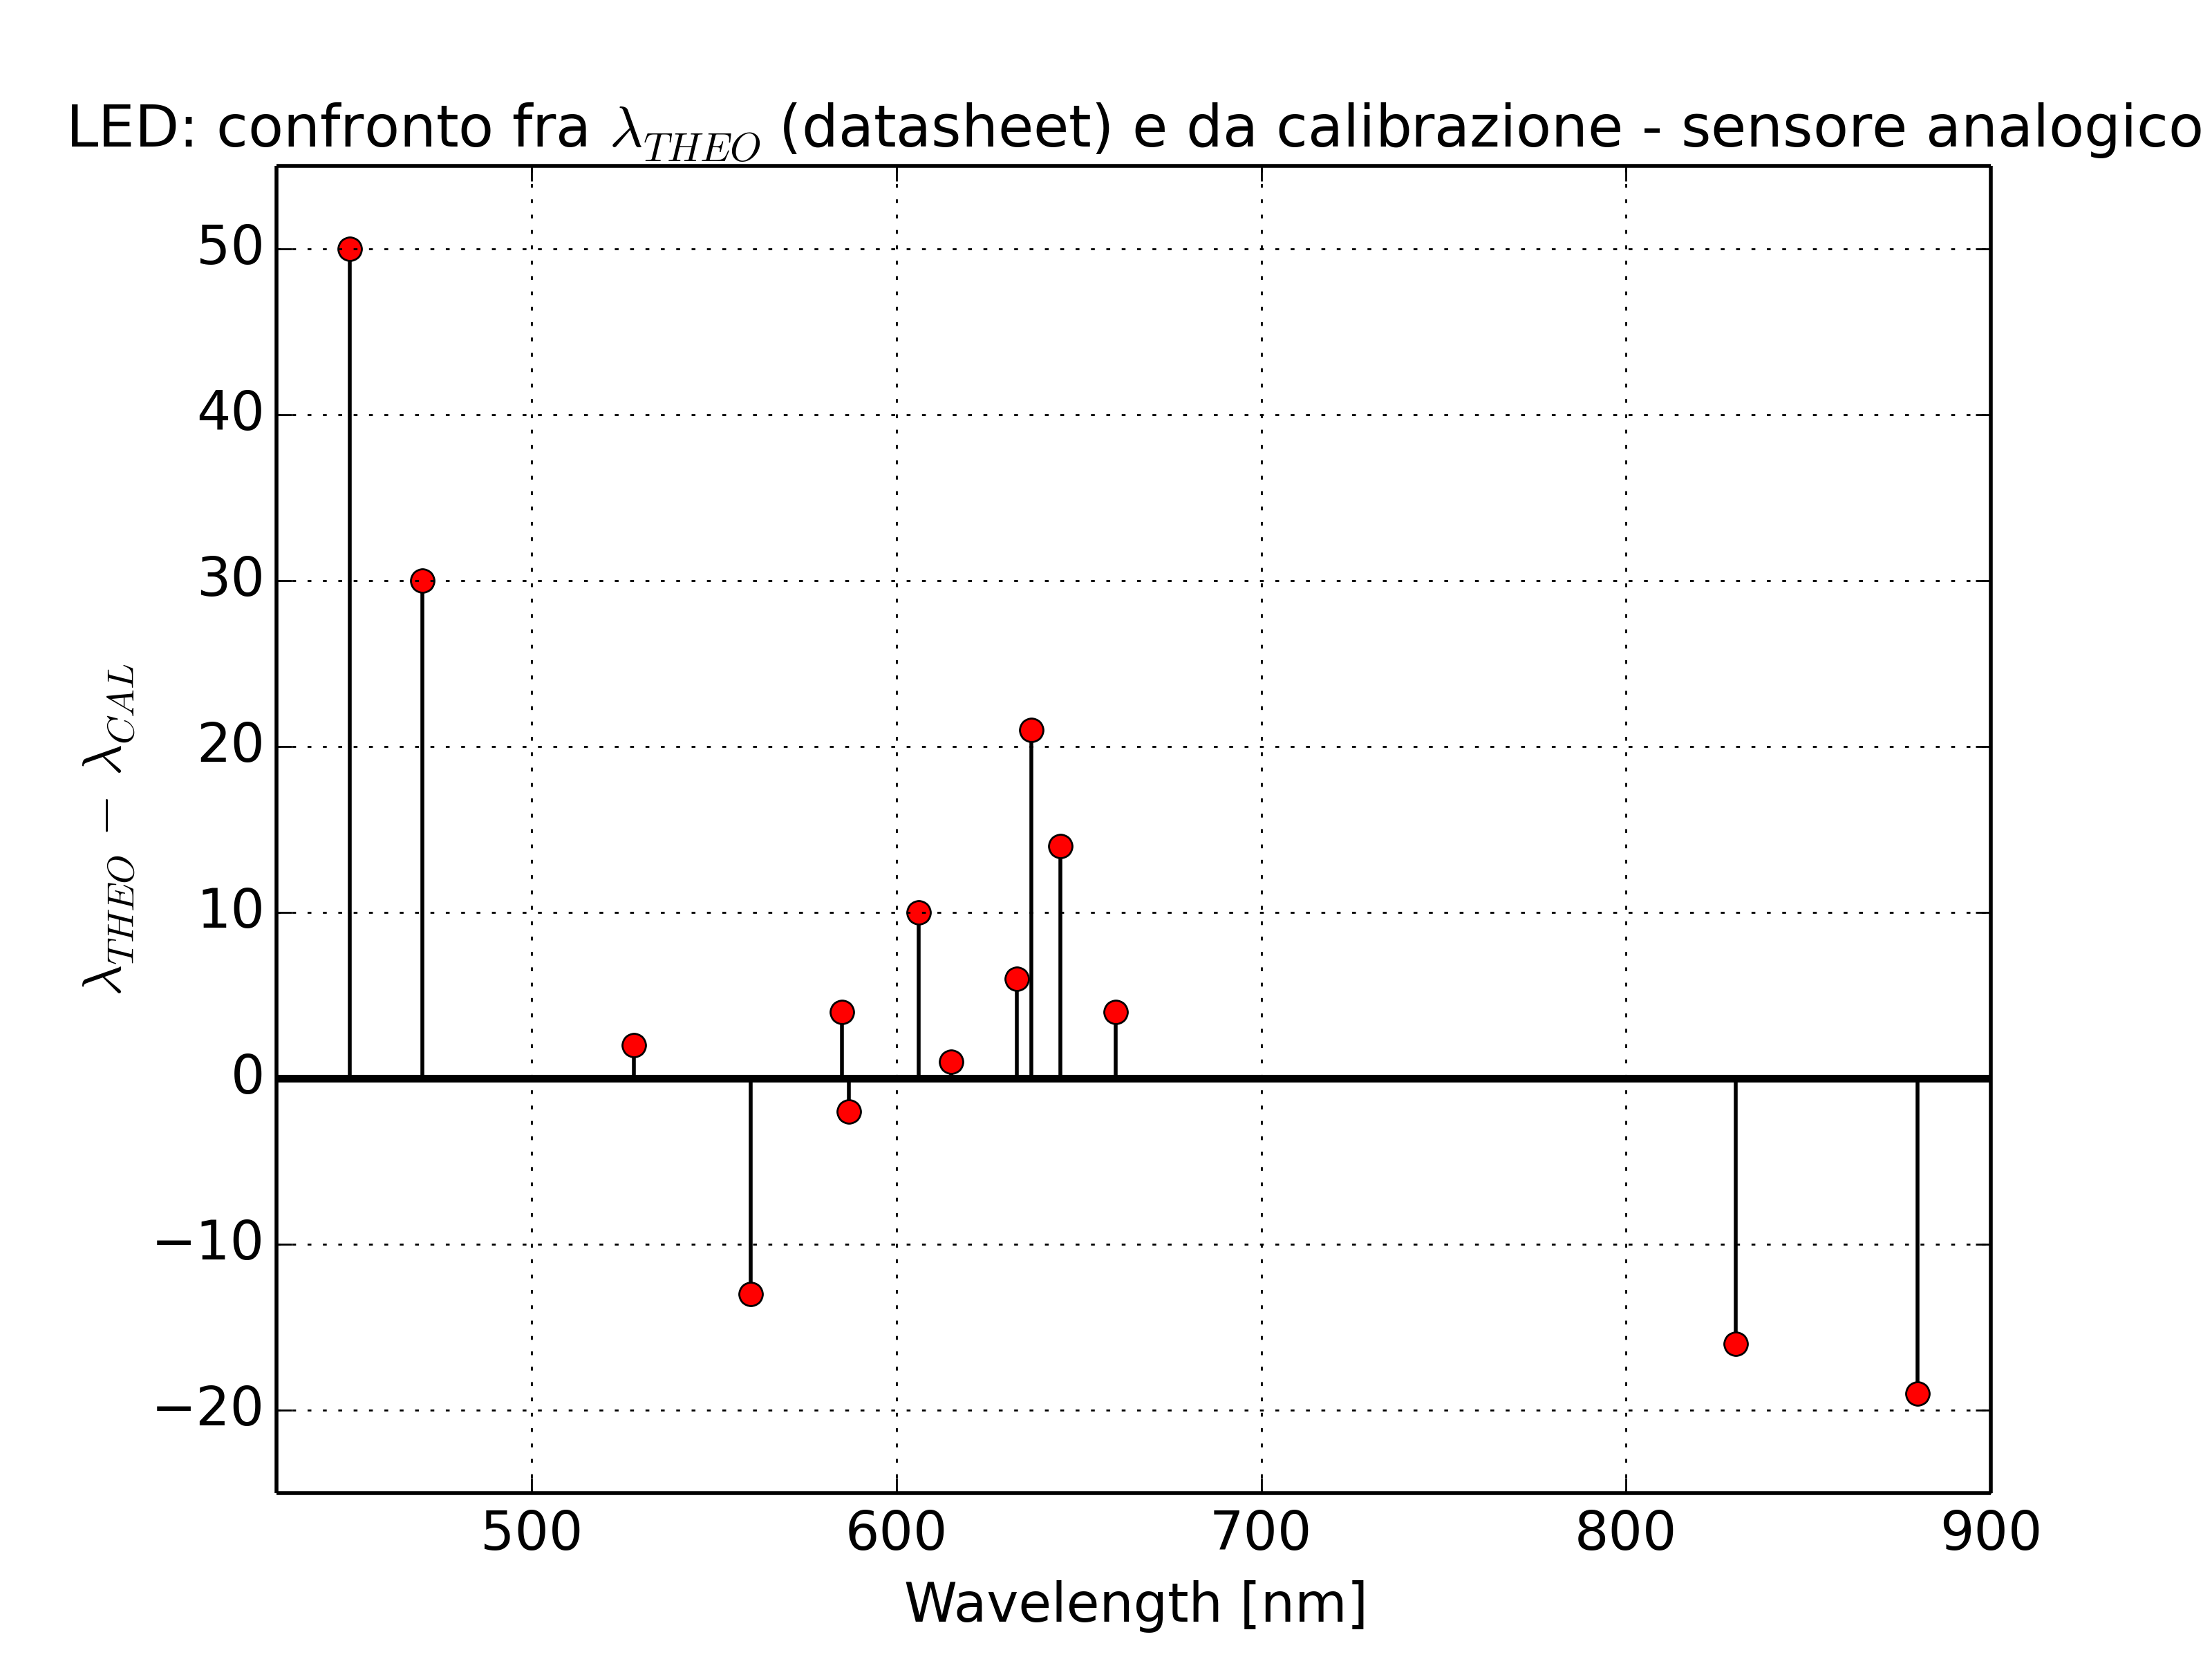
\includegraphics[width=0.4\linewidth]{./LED_confronto}
\label{fig:LED_confronto}}

\end{figure}


\begin{itemize}
\item Per i LED nel blu, la curva di calibrazione non copre valori di interesse.
\end{itemize}

\end{frame}




\begin{frame}{Estrapolazione della curva}
Vogliamo avere a disposizione dei valori attendibili nella regione 450-500nm.
\begin{itemize}
\item Per mezzo di Octave cerchiamo un polinomio interpolatore dei punti di calibrazione e prolunghiamolo per $\lambda$ fra 450-500nm. \item Funzione di interpolazione: \textsc{polyfit}. Di che grado? Comportamento estremamente variabile.
\item Ci aiutiamo modellizzando le curve di responsività come gaussiane.
\end{itemize}


\begin{figure}
\centering
\subfloat[Modellizzazione della curva di responsività: la curva in rosso è il log del rapporto.]{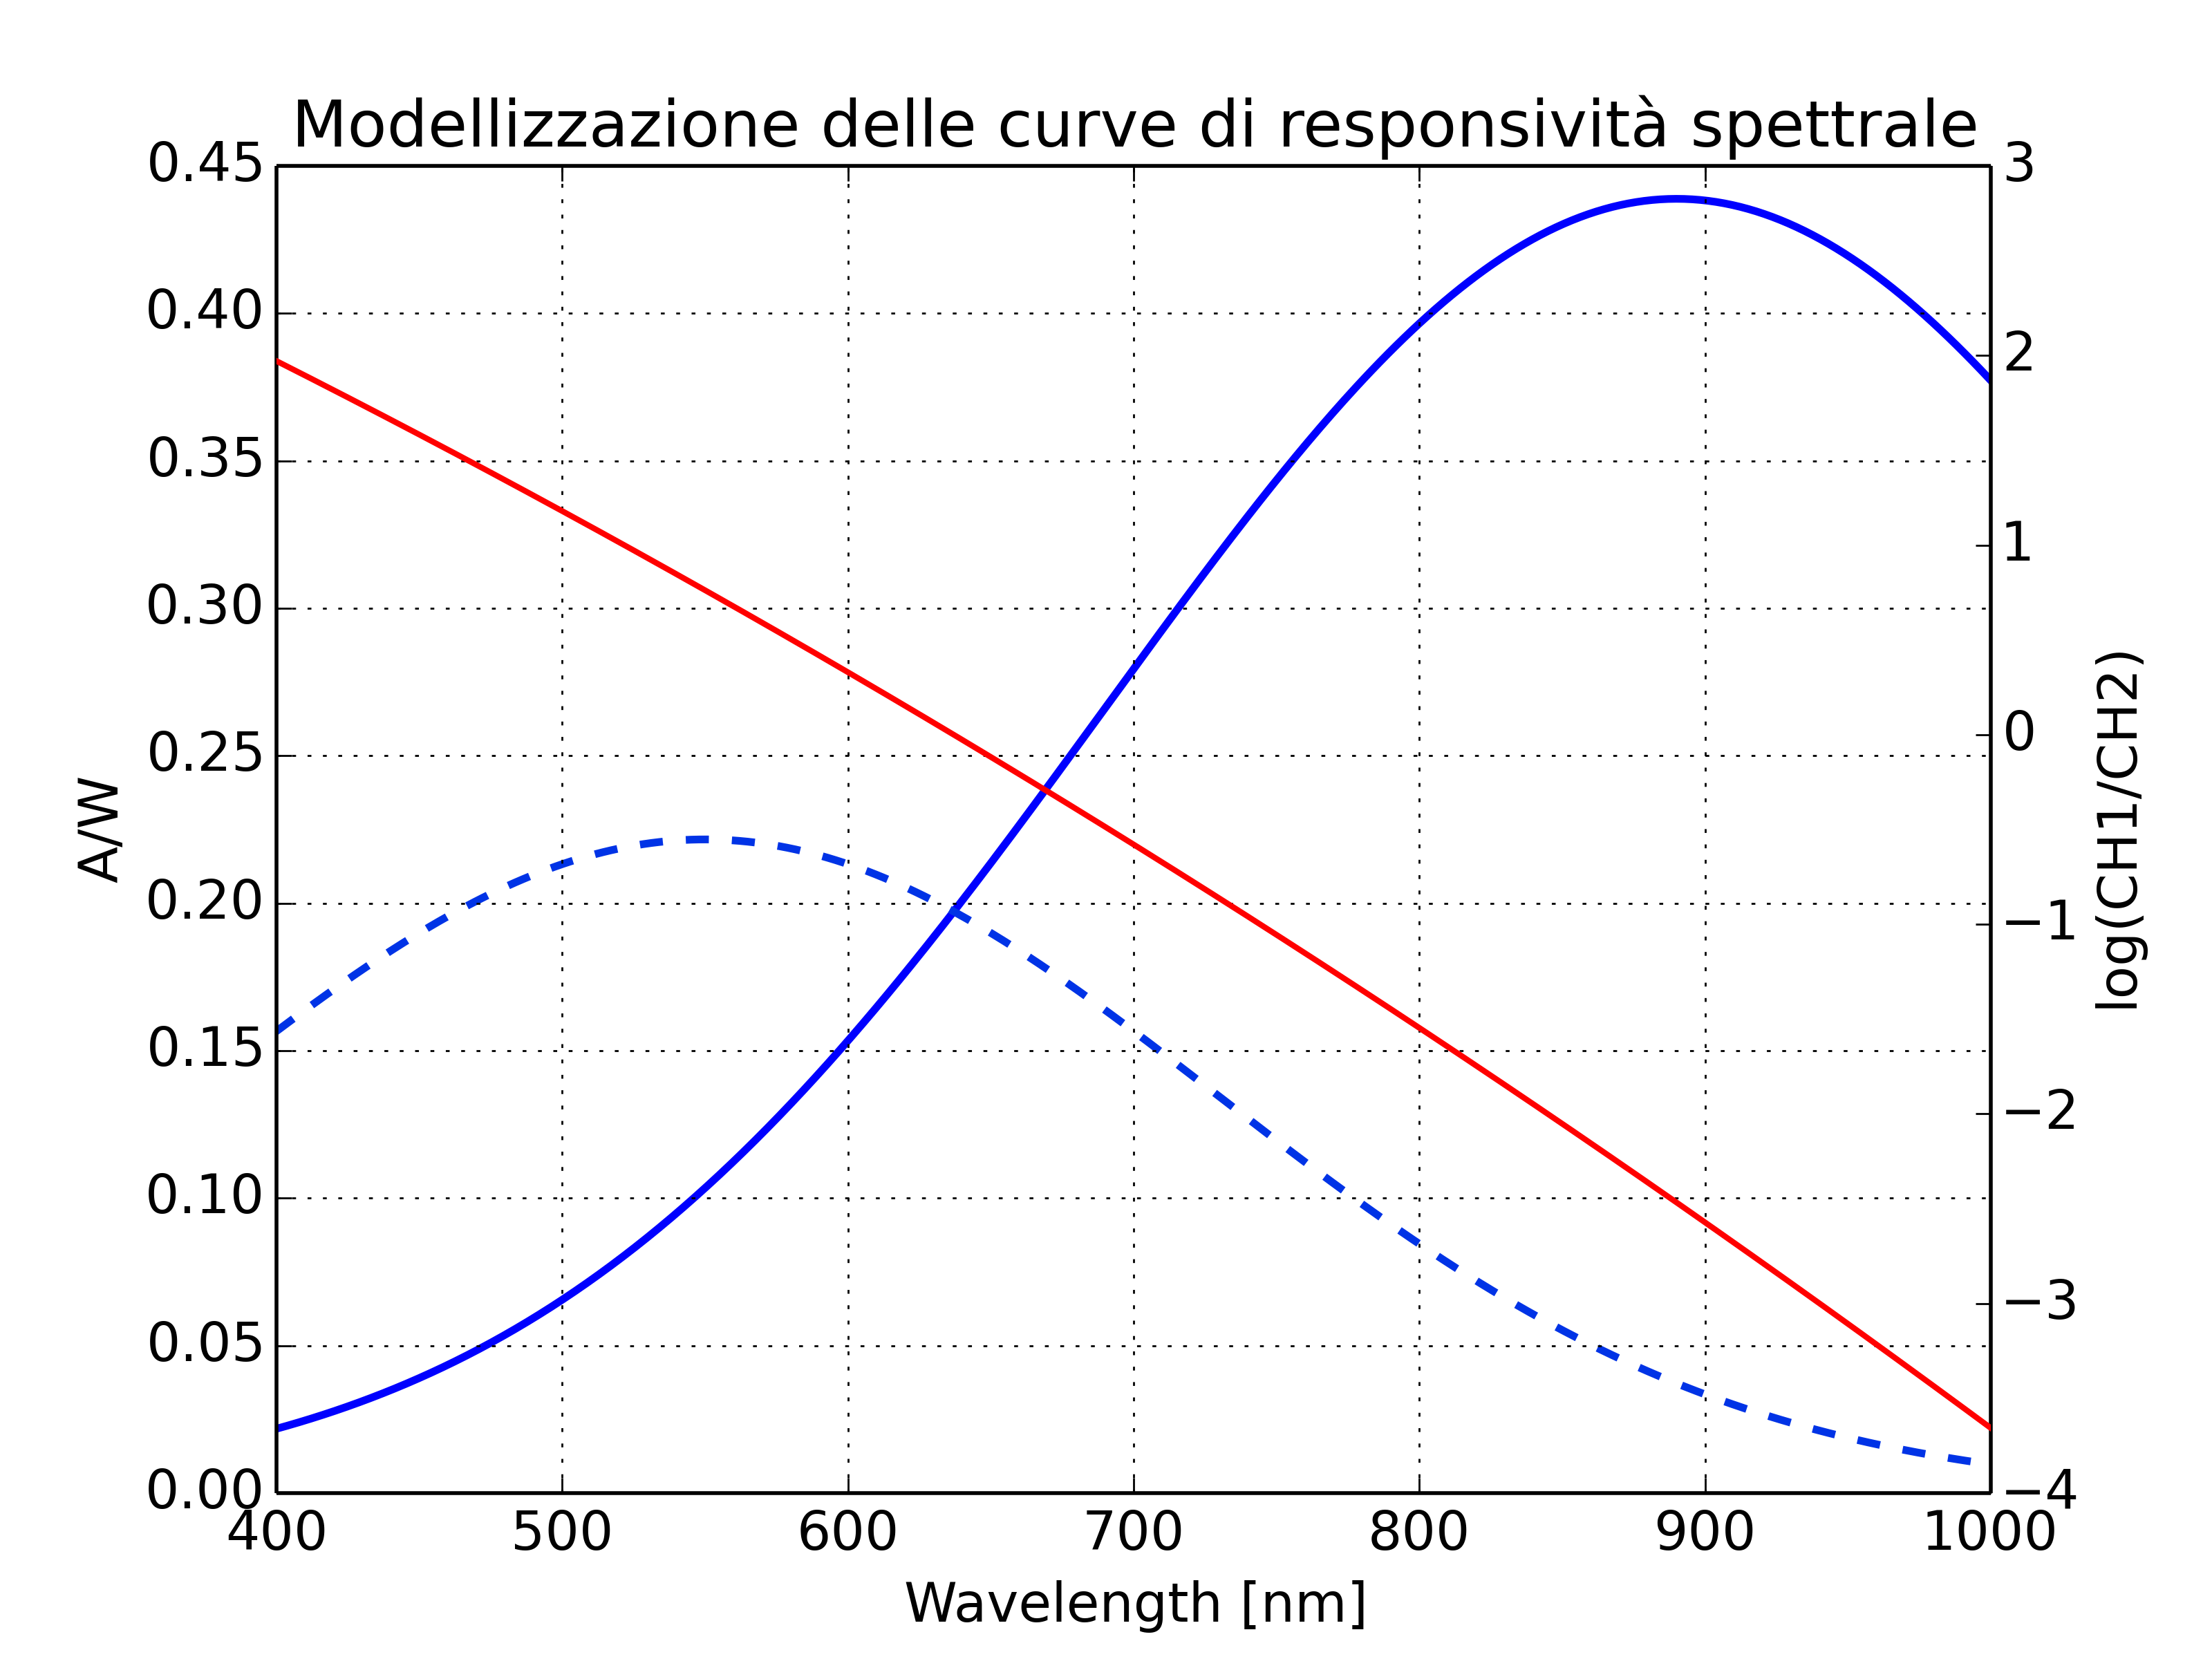
\includegraphics[width=0.4\linewidth]{./normal_respons}

\label{fig:normal_respons}}

\subfloat[Curva di responsività spettrale dei due diodi.]{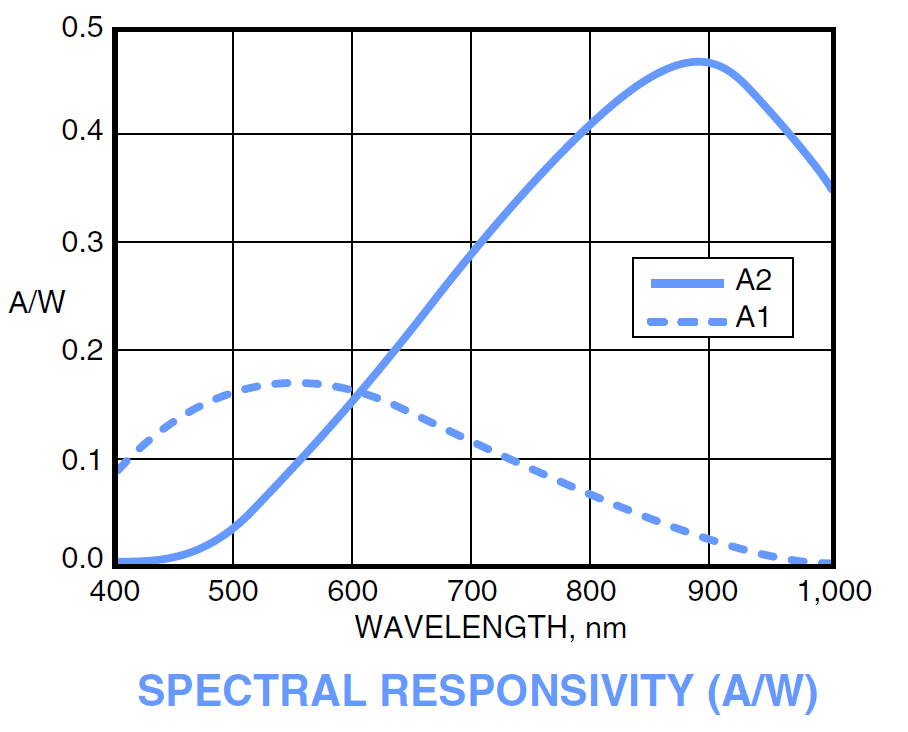
\includegraphics[width=0.4\linewidth]{./spectral_respo}
\label{fig:spectral_respo}}
\end{figure}


\end{frame}
\end{document}